\documentclass[a4paper,12pt]{article}
\usepackage{amsmath}
\usepackage{amssymb}
\usepackage[polish]{babel}
\usepackage{polski}
\usepackage[utf8]{inputenc}
\usepackage{indentfirst}
\usepackage{geometry}
\usepackage{array}
\usepackage[pdftex]{color,graphicx}
\usepackage{subfigure}
\usepackage{afterpage}
\usepackage{setspace}
\usepackage{color}
\usepackage{wrapfig}
\usepackage{listings}
\usepackage{datetime}


\renewcommand{\onehalfspacing}{\setstretch{1.6}}

\geometry{tmargin=2.5cm,bmargin=2.5cm,lmargin=2.5cm,rmargin=2.5cm}
\setlength{\parindent}{1cm}
\setlength{\parskip}{0mm}

\newenvironment{lista}{
\begin{itemize}
  \setlength{\itemsep}{1pt}
  \setlength{\parskip}{0pt}
  \setlength{\parsep}{0pt}
}{\end{itemize}}

\newcommand{\linia}{\rule{\linewidth}{0.4mm}}

\definecolor{lbcolor}{rgb}{0.95,0.95,0.95}
\lstset{
    backgroundcolor=\color{lbcolor},
    tabsize=4,
  language=C++,
  captionpos=b,
  tabsize=3,
  frame=lines,
  numbers=left,
  numberstyle=\tiny,
  numbersep=5pt,
  breaklines=true,
  showstringspaces=false,
  basicstyle=\footnotesize,
  identifierstyle=\color{magenta},
  keywordstyle=\color[rgb]{0,0,1},
  commentstyle=\color{Darkgreen},
  stringstyle=\color{red}
  }
\begin{document}

\noindent
\begin{tabular}{|c|p{11cm}|c|} \hline 
Grupa 1 & Kamil Sacha, Konrad Szwedo & \ddmmyyyydate\today \tabularnewline
\hline 
\end{tabular}

\renewcommand{\lstlistingname}{Listing kodu}

\section*{Zadanie 3 - Mnożenie macierzy GPU}

Naszym zadaniem było napisanie programu obliczającego wartość macierzy  \(C = A \times B\) gdzie macierze \(A, B, C\) są kwadratowe oraz posiadają rozmiar \(n \times n\) gdzie \(n\) jest potęgą 2. Program w celu przyśpieszenia obliczeń miał zostać stworzony w oparciu o środowisko Nvidia{\textregistered} CUDA\texttrademark{ }


\section*{Rozwiązanie problemu}

	Generowanie oraz proces obliczeń macierzy został przeniesiony z hosta (programu który wywołujemy na CPU) na proces graficzny, w związku z tym potrzebne było napisanie funkcji generujących i obliczających wynik mnożenia na karcie grafiki. 
	

\subsection*{Definiowanie rozmiarów siatki i bloku}	
	Pierwszym ważnym krokiem do rozpoczęcia obliczeń, jest zdefiniowanie odpowiednich rozmiarów siatki, oraz bloku 
	(jako blok definiujemy ilość wątków indeksowanych 2-wymiarowo). W naszym programie zastosowaliśmy taki algorytm wybierania siatki tak aby rozmiar x oraz y (gdzie x to ilość bloków w płaszczyźnie poziomej a y pionowej) był zawsze wielokrotnością 16. 
	Wymiary bloku zostały ustawione na sztywno \( 16 \times 16\) (rozmiar ten został dobrany eksperymentalnie).
Blok ten został  użyty również do metody generowania macierzy \(A,B\) \textbf{matrixMultiplyKernel(...)} która to generuje macierze z podanych wzorów zapisując przy użyciu tablic alokowanych na GPU.
	
	
\begin{lstlisting}[caption=Algorytm podziału na siatkę i bloki.=GPU_KERNEL]
 
dim3 threadsPerBlock(BLOCK_SIZE, BLOCK_SIZE);

dim3 grid( (int) ceil(cpu_A.matrixSize / (float)threadsPerBlock.x), 
           (int) ceil(cpu_A.matrixSize / (float)threadsPerBlock.y));
	
\end{lstlisting}	
	
	 Dla przykładu: gdy wejściowe macierze \(A, B\) będą wymiarów \(12 \times 12\) wtedy siatka będzie wymiarów \( 3 \times 3 \) ponieważ zaokrąglamy w górę \(33 \div 16 = 2.065\) (zaokrąglamy w górę do 3).
	
	
	
\subsection*{Algorytm mnożenia}

Funkcja jądra obliczająca wynik mnożenia, została uproszczona do minimum w celu łatwego przeglądania kodu oraz przyśpieszenia obliczeń. 
Działa ona tak, że każda komórka macierzy C ma swój odpowiednik w utworzonym przez środowisko wątku.
 Każdy wątek odpowiedzialny jest za wymnożenie całego wiersza macierzy A z odpowiednią kolumną macierzy B.
W tym celu są nam potrzebne indeksy dzięki którym możemy zidentyfikować dany wątek w odniesieniu do macierzy.
 Zostało również zapisane zabezpieczenie, przed wyjściem poza zakres. 
 Taka sytuacja zdarzy się zawszę, gdy rozmiar macierzy nie będzie liczbą podzielną przez 16. 
W przypadku braku takiego warunku, w sytuacji powyżej, funkcja jądra próbowała by się odwołać do nie istniejących komórek macierzy co spowodowałoby błąd w czasie uruchomienia. 
Dodatkowo zostały użyte pomocnicze funkcję \textbf{getElement} oraz \textbf{setElement} które poprawiają czytelność kodu.


\begin{lstlisting}[caption=Główna funkcja jądra GPU - Mnożenie macierzy.=GPU_KERNEL] 
__global__ void matrixMultiplyKernel(Matrix A, Matrix B, Matrix C) {

	int row = threadIdx.y + blockIdx.y * blockDim.y;
	int col = threadIdx.x + blockIdx.x * blockDim.x;

	int matrixSize = A.matrixSize;

	float tempCValue = 0.0f;

	if (row < matrixSize && col < matrixSize){

		for(int k = 0; k < matrixSize; k++) {
			tempCValue += GetElement(A, row, k) * GetElement(B, k, col);
		}

		SetElement(C, row, col, tempCValue);
	}
}
\end{lstlisting}

\section*{Wyniki i wnioski}

Testy zostały przeprowadzone na serwerze cuda.iti.pk.edu.pl, przy użyciu jednej karty graficznej Nvidia\textregistered GTX480. Z wykresu możemy zauważyć, że największą wydajność uzyskujemy dla bloku o wymiarach \( 16 \times 16\). 

\begin{figure}

	\begin{center}

 		% GNUPLOT: LaTeX picture with Postscript
\begingroup
  \makeatletter
  \providecommand\color[2][]{%
    \GenericError{(gnuplot) \space\space\space\@spaces}{%
      Package color not loaded in conjunction with
      terminal option `colourtext'%
    }{See the gnuplot documentation for explanation.%
    }{Either use 'blacktext' in gnuplot or load the package
      color.sty in LaTeX.}%
    \renewcommand\color[2][]{}%
  }%
  \providecommand\includegraphics[2][]{%
    \GenericError{(gnuplot) \space\space\space\@spaces}{%
      Package graphicx or graphics not loaded%
    }{See the gnuplot documentation for explanation.%
    }{The gnuplot epslatex terminal needs graphicx.sty or graphics.sty.}%
    \renewcommand\includegraphics[2][]{}%
  }%
  \providecommand\rotatebox[2]{#2}%
  \@ifundefined{ifGPcolor}{%
    \newif\ifGPcolor
    \GPcolortrue
  }{}%
  \@ifundefined{ifGPblacktext}{%
    \newif\ifGPblacktext
    \GPblacktextfalse
  }{}%
  % define a \g@addto@macro without @ in the name:
  \let\gplgaddtomacro\g@addto@macro
  % define empty templates for all commands taking text:
  \gdef\gplbacktext{}%
  \gdef\gplfronttext{}%
  \makeatother
  \ifGPblacktext
    % no textcolor at all
    \def\colorrgb#1{}%
    \def\colorgray#1{}%
  \else
    % gray or color?
    \ifGPcolor
      \def\colorrgb#1{\color[rgb]{#1}}%
      \def\colorgray#1{\color[gray]{#1}}%
      \expandafter\def\csname LTw\endcsname{\color{white}}%
      \expandafter\def\csname LTb\endcsname{\color{black}}%
      \expandafter\def\csname LTa\endcsname{\color{black}}%
      \expandafter\def\csname LT0\endcsname{\color[rgb]{1,0,0}}%
      \expandafter\def\csname LT1\endcsname{\color[rgb]{0,1,0}}%
      \expandafter\def\csname LT2\endcsname{\color[rgb]{0,0,1}}%
      \expandafter\def\csname LT3\endcsname{\color[rgb]{1,0,1}}%
      \expandafter\def\csname LT4\endcsname{\color[rgb]{0,1,1}}%
      \expandafter\def\csname LT5\endcsname{\color[rgb]{1,1,0}}%
      \expandafter\def\csname LT6\endcsname{\color[rgb]{0,0,0}}%
      \expandafter\def\csname LT7\endcsname{\color[rgb]{1,0.3,0}}%
      \expandafter\def\csname LT8\endcsname{\color[rgb]{0.5,0.5,0.5}}%
    \else
      % gray
      \def\colorrgb#1{\color{black}}%
      \def\colorgray#1{\color[gray]{#1}}%
      \expandafter\def\csname LTw\endcsname{\color{white}}%
      \expandafter\def\csname LTb\endcsname{\color{black}}%
      \expandafter\def\csname LTa\endcsname{\color{black}}%
      \expandafter\def\csname LT0\endcsname{\color{black}}%
      \expandafter\def\csname LT1\endcsname{\color{black}}%
      \expandafter\def\csname LT2\endcsname{\color{black}}%
      \expandafter\def\csname LT3\endcsname{\color{black}}%
      \expandafter\def\csname LT4\endcsname{\color{black}}%
      \expandafter\def\csname LT5\endcsname{\color{black}}%
      \expandafter\def\csname LT6\endcsname{\color{black}}%
      \expandafter\def\csname LT7\endcsname{\color{black}}%
      \expandafter\def\csname LT8\endcsname{\color{black}}%
    \fi
  \fi
  \setlength{\unitlength}{0.0500bp}%
  \begin{picture}(7200.00,5040.00)%
    \gplgaddtomacro\gplbacktext{%
      \csname LTb\endcsname%
      \put(1078,704){\makebox(0,0)[r]{\strut{} 1000}}%
      \csname LTb\endcsname%
      \put(1078,1111){\makebox(0,0)[r]{\strut{} 1500}}%
      \csname LTb\endcsname%
      \put(1078,1518){\makebox(0,0)[r]{\strut{} 2000}}%
      \csname LTb\endcsname%
      \put(1078,1925){\makebox(0,0)[r]{\strut{} 2500}}%
      \csname LTb\endcsname%
      \put(1078,2332){\makebox(0,0)[r]{\strut{} 3000}}%
      \csname LTb\endcsname%
      \put(1078,2740){\makebox(0,0)[r]{\strut{} 3500}}%
      \csname LTb\endcsname%
      \put(1078,3147){\makebox(0,0)[r]{\strut{} 4000}}%
      \csname LTb\endcsname%
      \put(1078,3554){\makebox(0,0)[r]{\strut{} 4500}}%
      \csname LTb\endcsname%
      \put(1078,3961){\makebox(0,0)[r]{\strut{} 5000}}%
      \csname LTb\endcsname%
      \put(1078,4368){\makebox(0,0)[r]{\strut{} 5500}}%
      \csname LTb\endcsname%
      \put(1078,4775){\makebox(0,0)[r]{\strut{} 6000}}%
      \csname LTb\endcsname%
      \put(1210,484){\makebox(0,0){\strut{} 0}}%
      \csname LTb\endcsname%
      \put(1909,484){\makebox(0,0){\strut{} 2}}%
      \csname LTb\endcsname%
      \put(2608,484){\makebox(0,0){\strut{} 4}}%
      \csname LTb\endcsname%
      \put(3307,484){\makebox(0,0){\strut{} 6}}%
      \csname LTb\endcsname%
      \put(4007,484){\makebox(0,0){\strut{} 8}}%
      \csname LTb\endcsname%
      \put(4706,484){\makebox(0,0){\strut{} 10}}%
      \csname LTb\endcsname%
      \put(5405,484){\makebox(0,0){\strut{} 12}}%
      \csname LTb\endcsname%
      \put(6104,484){\makebox(0,0){\strut{} 14}}%
      \csname LTb\endcsname%
      \put(6803,484){\makebox(0,0){\strut{} 16}}%
      \put(176,2739){\rotatebox{-270}{\makebox(0,0){\strut{}Średni czas wykonania [ms]}}}%
      \put(4006,154){\makebox(0,0){\strut{}Ilość wątków}}%
    }%
    \gplgaddtomacro\gplfronttext{%
      \csname LTb\endcsname%
      \put(5816,4602){\makebox(0,0)[r]{\strut{}Czas wykonania}}%
    }%
    \gplbacktext
    \put(0,0){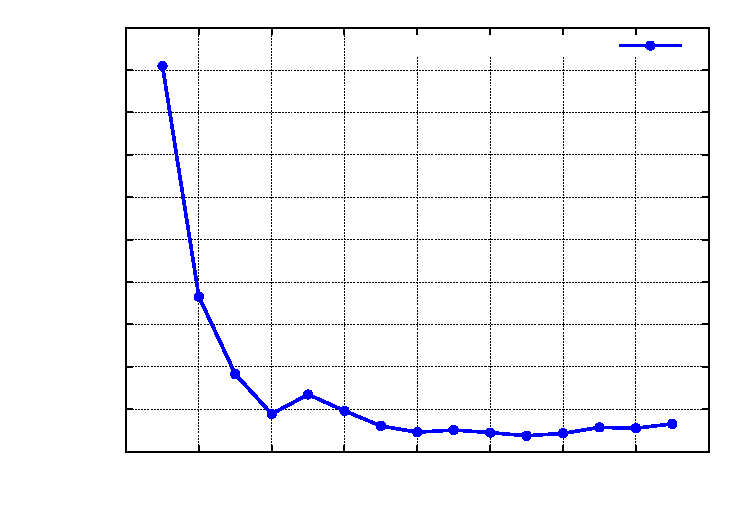
\includegraphics{wykres_czasu}}%
    \gplfronttext
  \end{picture}%
\endgroup
   		
 		
	\end{center}


    \caption{Wykres zależności czasu wykonania od rozmiaru bloku \(n \times n\). Dla macierzy \( A, B, C\) o wymiarach \(8192 \times 8192\) elementów.}
\end{figure}



Maksymalny rozmiar bloku jaki możemy utworzyć to taki który posiada maksimum 1024 wątki (np \( 32 \times 32\)). Najlepszy czas uzyskaliśmy dla bloku rozmiarów: \(16 \times 16\) wywołanie samej funkcji jądra odpowiedzialnej za wymnożenie macierzy to około 13772ms czyli 13s. 
Najgorszy czas został uzyskany dla rozmiaru bloku \(2 \times 2\), jest to związane z tym, że jednostki procesujące musiały uruchamiać maksimum 4 wątki na blok, co jest niewykorzystywaniem zasobów jednostek streamujących SM. 
(SM są przystosowane do dużej ilości wątków gdyż są one zarządzane sprzętowo i nie występuje narzut związany z np. wywłaszczaniem, tworzeniem, zarządzaniem).



\end{document}